% vim: spell spelllang=en_gb
\chapter{Methods}

This section discusses and motivates the methods used in the project. Figure \ref{fig:flow_chart}
shows a flow chart of the pipeline (an enlarged copy is available in Figure \ref{fig:flow_chart_big}
of Appendix \ref{appendix:raw}). The pipeline consists of the following steps: Data collection, text
classification, location extraction, and visualization. Python is the primary programming language
used for the project because of the rich ecosystem surrounding it, especially when it comes to data
science-related tasks. The code base is available at a GitHub
repository\footnote{https://github.com/YasserKa/Classification-and-visualization-of-natural-disasters-using-Twitter}
accompanied with a \texttt{README.md} containing instructions to set up the environment and run the
project.

\begin{figure}[H]
\begin{center}
  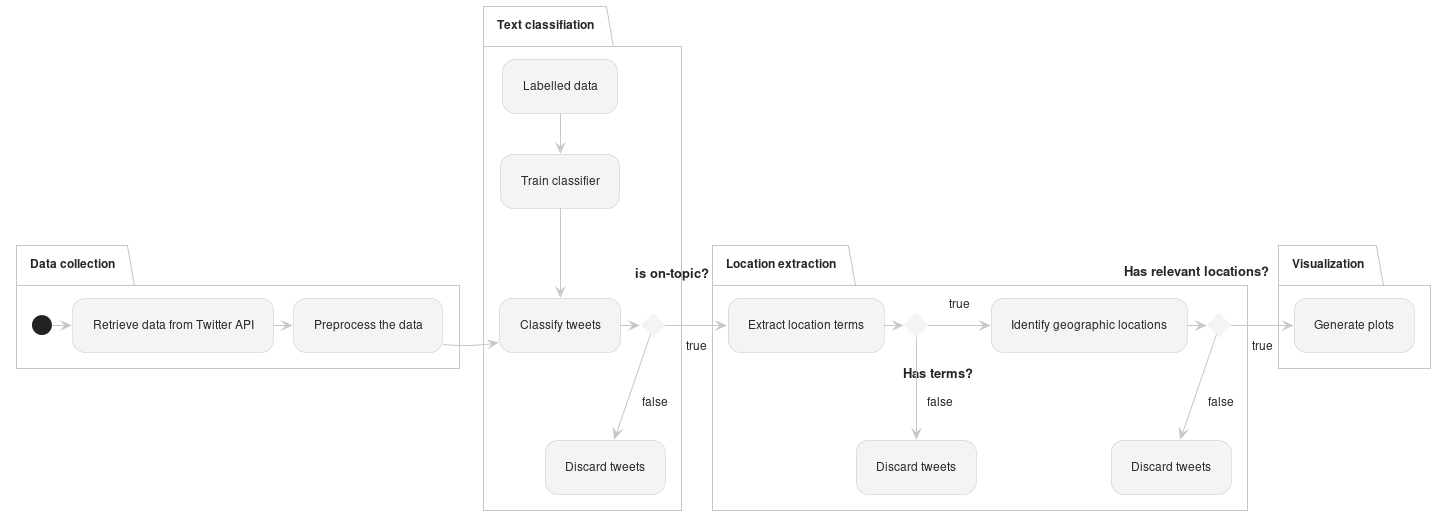
\includegraphics[width=\columnwidth]{./images/pipeline.png}
\end{center}
\caption{Flow chart for the pipeline}
\label{fig:flow_chart}
\end{figure}

\section{Data Collection}

Finding a good quality data source is the first step to having a lean start for most research
questions. The pipeline trains an \ac{ML} classifier using a manually labelled dataset containing
4899 tweets with attributes presented in Table~\ref{tab:dataset_attr}. The text and metadata of the tweets are extracted
from Twitter's API using the IDs. The trained model performance is verified using the tweets from
the API using Tweepy\footnote{https://docs.tweepy.org/en/latest/index.html}, a python library for
accessing Twitter API.

\begin{table}
  \center
  \label{tab:dataset_attr}
  \begin{tabular}{|l|l|l|}
    \hline
    Field & Type & Description \\
    \hline
    ID & Int & ID of the tweet\\
    \hline
    On Topic  & Bool & Text discusses an event \\
    \hline
    Informative sarcastic  & Bool & Text contains relevant information about the event \\
    \hline
    Contains IMPACT info & Bool & Text discusses the impact of the event \\
    \hline
    Explicit location & Bool & Text mentions the location of the event \\
    \hline
  \end{tabular}
  \caption{Dataset attributes}
\end{table}

Textual data requires pre-processing for several tasks, such as training an \ac{ML} algorithm, text
analysis, and visualization. Parts of text that don't contribute to the context are removed:
\ac{URL}s, emojis, mentions, hashtag signs, numbers, new lines, punctuation, and stopwords (provided
by spaCy\footnote{https://spacy.io/}, an \ac{NLP} python library). Afterwards, duplicate tweets,
tweets containing no text, and retweets are discarded from the dataset.

Data needs to be stored and managed to accommodate policies and regulations. Twitter's developer
policy\footnote{https://developer.twitter.com/en/developer-terms/policy} has a content
redistribution section stating that only the IDs of the tweets can be shared online. Thus, the
tweets can't be available publicly on such as GitHub, the service that hosts the publicly available
code base. To this end, the data is stored and cached after each step on google drive using
\ac{DVC}'s\footnote{https://dvc.org/doc} data management capabilities.


Twitter's API provides an extensive list of information about the
tweets\footnote{https://developer.twitter.com/en/docs/twitter-api/data-dictionary/object-model/tweet}.
It shares the engagement metrics of the tweet, including like count, reply count, and retweet count;
as well as, an \ac{NLP} analysis of its own, such as the language used, and entities parsed from the
text. Table~\ref{tab:tweet_attr} shows the tweet's attributes used in this project for the following reasons: the id to
generate the \ac{URL} of the tweet, the text for \ac{NLP} tasks, the created date for temporal
analysis, and the author id to reduce spam.

\begin{table}
  \center
  \label{tab:tweet_attr}
  \begin{tabular}{|l|l|l|}
    \hline
    Attribute & Type & Description \\
    \hline
    id & Int & The unique identifier of the requested Tweet \\
    \hline
    text & Str & The actual UTF-8 text of the Tweet \\
    \hline
    created at & Date  & Creation time of the Tweet \\
    \hline
    author id & Str & The unique identifier of the tweet creator \\
    \hline
  \end{tabular}
  \caption{Tweet attributes used}
\end{table}

\section{Text Classification}

There are three groups of approaches for \ac{NLP} tasks: heuristics, \ac{ML}, and deep
learning. The heuristics approach is the oldest one which builds rules manually for a specific task
by using dictionaries and thesauruses. \ac{ML} techniques, including probabilistic
modelling and likelihood maximization, are used on a numerical representation of the textual data to
learn a model. Neural networks are a popular choice for handling complex, and unstructured data,
making them a suitable candidate for language.

\ac{RNN} \cite{hopfieldNeuralNetworksPhysical1982} is a common artificial neural network for
\ac{NLP} tasks, such as text classification, \ac{NER}, and machine translation. Its memory enables
it to take information from previous input to update the current input and output vector (called
hidden state) as shown in Figure~\ref{fig:rnn_example}, making it appropriate for sequential. For common
tasks such as translation  an encoder-decoder architecture is needed, where the encoder encodes the
input sequence into a numerical representation (called the last hidden state) that gets passed to
the decoder for output sequence generation. Figure~\ref{fig:rnn_encoder_decoder} shows an example of translating the
English statement ``Transformers are great!'' to the German language. \ac{RNN} has shortcomings when it tries to
capture the context for long sequences of information, where the encoder might lose the information
at the start of the sequence while forming the representation. \ac{RNN}'s  weak memory can be
addressed by using the attention mechanism that allows the decoder to access all the hidden states
of the encoder. The main goal of attention is to enable the decoder to prioritize the states using
weights it assigns at every decoding timestamp. Figure~\ref{fig:rnn_encoder_decoder_attention} shows
an example for predicting the third token in the output sequence. Even though attention improves the
accuracy of the translations, the computations are sequential and cannot be parallelized.

% The trims are added to remove the black edges
\begin{figure}[H]
\begin{center}
  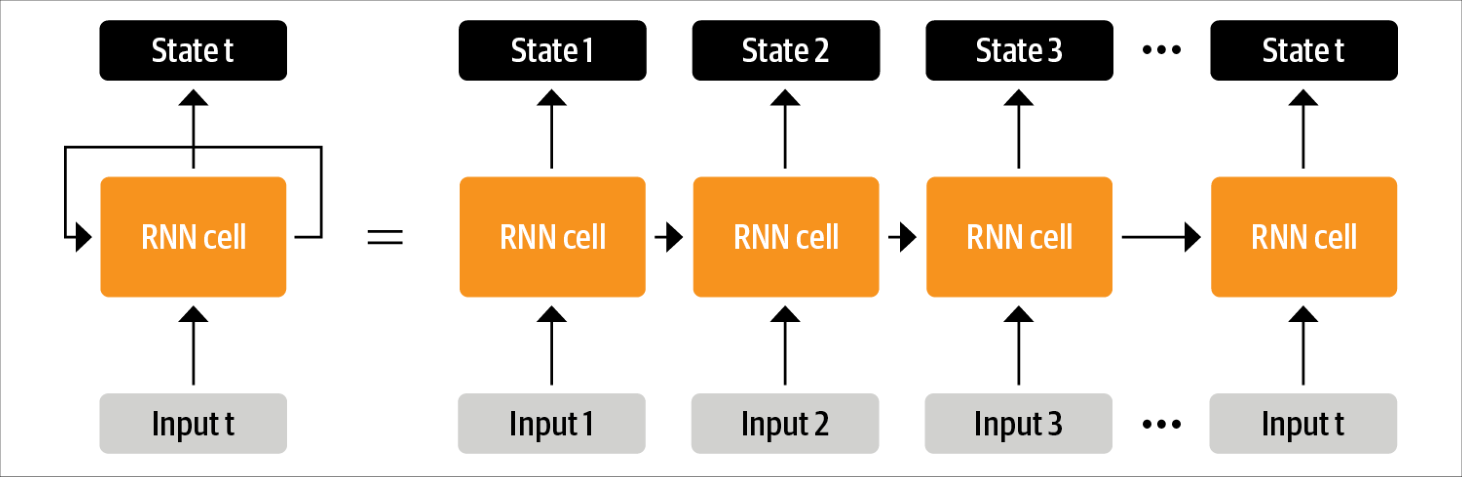
\includegraphics[width=\columnwidth,trim={0.1cm 0.1cm 0.1cm 0.1cm},clip]{./images/unrolling_rnn.png}
\end{center}
\caption{RNN example \cite{tunstallNaturalLanguageProcessing2022}}
\label{fig:rnn_example}
\end{figure}

\begin{figure}[H]
\begin{center}
  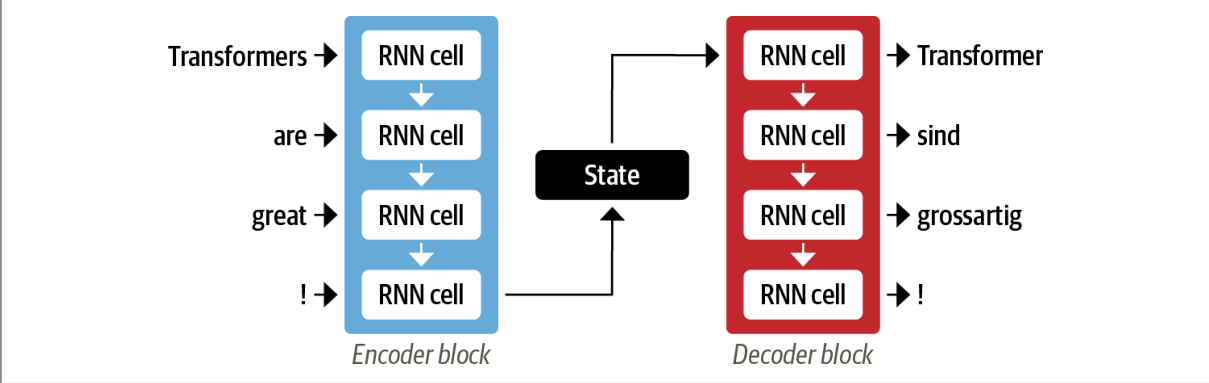
\includegraphics[width=\columnwidth, trim={0.1cm 0.1cm 0.1cm 0.1cm},clip]{./images/encoder-decoder_rnn.png}
\end{center}
\caption{Two \ac{RNN}s making an encoder-decoder architecture \cite{tunstallNaturalLanguageProcessing2022}}
\label{fig:rnn_encoder_decoder}
\end{figure}

\begin{figure}[H]
\begin{center}
  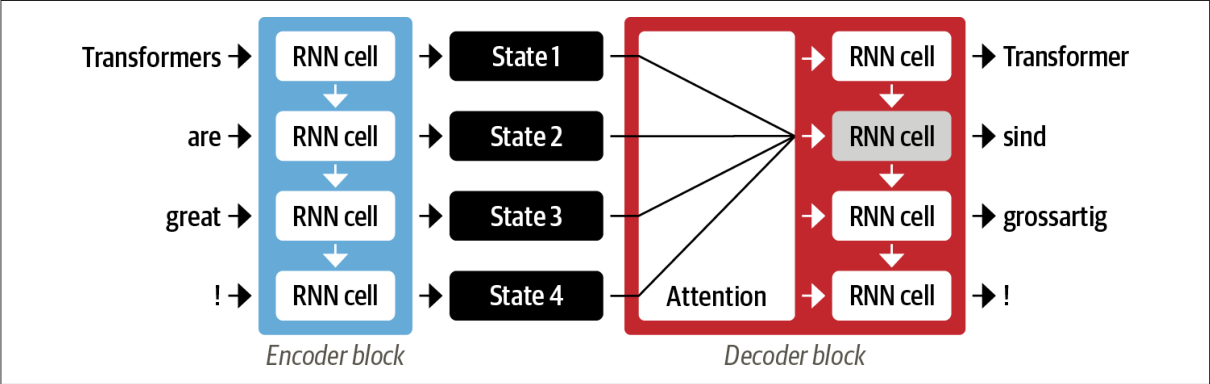
\includegraphics[width=\columnwidth,trim={0.1cm 0.1cm 0.1cm 0.1cm},clip]{./images/encoder-decoder_rnn_attention.png}
\end{center}
\caption{Two \ac{RNN}s making an encoder-decoder architecture with attention mechanism \cite{tunstallNaturalLanguageProcessing2022}}
\label{fig:rnn_encoder_decoder_attention}
\end{figure}

Transformers with its self-attention architecture, proposed by google researchers
\cite{vaswaniAttentionAllYou2017}, made the training process much faster. The idea is to use
attention on all states in the same layer of the neural network.
Figure~\ref{fig:encoder_decoder_transformer} shows the self-attention mechanism on both encoder
and decoder with their outputs fed to feed-forward neural networks. Transformers still require a
large amount of labelled text data to train the models,which gets circumvent using transfer learning
by pre-training a model on a huge dataset that gets fine-tuned afterwards on a much smaller dataset
for a more specific task.

\begin{figure}[H]
\begin{center}
  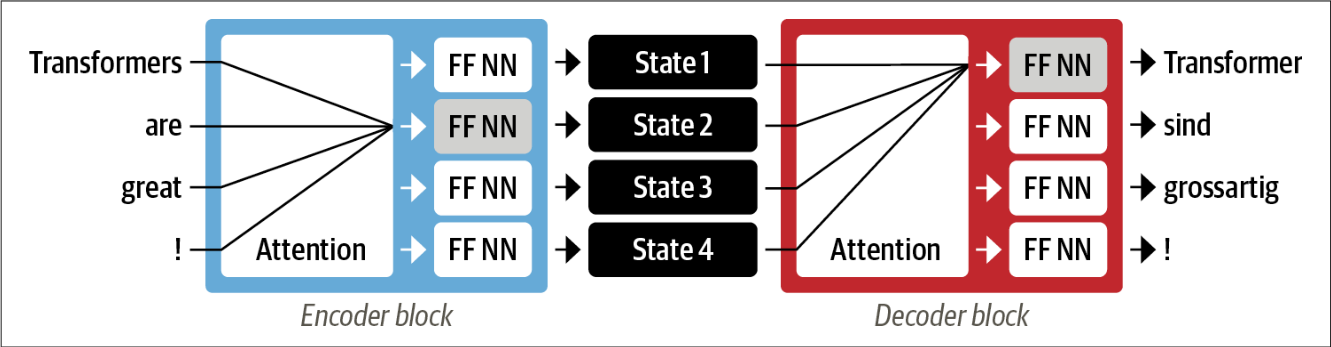
\includegraphics[width=\columnwidth, trim={0.1cm 0.1cm 0.1cm 0.1cm},clip]{./images/encoder-decoder_transformer.png}
\end{center}
\caption{Transformer's encoder-decoder architecture \cite{tunstallNaturalLanguageProcessing2022}}
\label{fig:encoder_decoder_transformer}
\end{figure}

This project uses the DistilBERT transformer\cite{Sanh2019DistilBERTAD}, a variant of BERT, for text
classification.  The main advantage of this model is that it achieves comparable performance to BERT
while being significantly smaller than BERT while being significantly smaller and more efficient. A
DistilBERT pre-trained model is provided by Hugging Face\footnote{https://huggingface.co/}, a
framework that provides a unified API for over more than 50 architectures, making it easier for
users to integrate \ac{NLP} models into their applications.

After pre-processing the data, there are several steps to obtain the trained model. DistilBERT works
on the English language, and since Sweden is the focus of the research, most of the text is in
Swedish; thus, the text is translated to English using google
translate\footnote{https://translate.google.com/} by a python library wrapper
deep-translate\footnote{https://deep-translator.readthedocs.io/en/latest/}. The text classification
purpose is to identify the tweets that discuss flood events, so the ``On Topic'' attribute of the
dataset is used as a label during training. The learning rate for the neural network is $5\times e^{-5}$ with
100 warmup steps over three epochs using 90\% of the labelled tweets as training data, 5\% as test
data, and 5\% for validation. Training the model locally takes a long time with the available
resources, so the training is done using Amazon
SageMaker\footnote{https://aws.amazon.com/sagemaker/}, a service that covers tools to build, train,
and deploy \ac{ML} models. The data is uploaded to Amazon Simple Storage Service (Amazon S3) to make it
accessible for the Hugging Face training script that is executed in an instance available in the
cloud. After the training is complete, the fine-tuned model and the evaluation metric are
downloaded. The evaluation metric consists of the following:

item
\begin{itemize}
  \item Accuracy: the fraction of the number of correctly classified instances (i.e., true positives
    and true negatives) among all instances (i.e., whole dataset) (equation~\ref{eq:accuracy}).
 \begin{equation}
   \text{Accuracy}=\frac{TN+TP}{TN+FN+TP+FP} 
   \label{eq:accuracy}
\end{equation}
\item Precision: the fraction of the number of correctly classified relevant instances (i.e., true
  positives) among the total number of instances classified as relevant (i.e., true positives and
  false positives) (equation~\ref{eq:precision}).
 \begin{equation}
   \text{Precision}=\frac{TP}{TP+FP} 
   \label{eq:precision}
\end{equation}
\item Recall: the fraction of the correctly classified relevant instances (i.e., true positives)
  among all relevant instances (i.e. true positives and false negatives) (equation~\ref{eq:recall}).
 \begin{equation}
   \text{Precision}=\frac{TP}{TP+FN} 
   \label{eq:recall}
\end{equation}
\item $\text{F}_1$ score: the harmonic mean of precision and recall (equation~\ref{eq:f1}).
 \begin{equation}
   \text{F}_1 =2.\frac{\text{Precision}.\text{Recall}}{\text{Precision}+\text{Recall}} 
   \label{eq:f1}
\end{equation}
\end{itemize}
  

  
